\documentclass[12pt, a4paper]{article}
\usepackage[margin = 1in]{geometry}
\usepackage{amsthm, amsmath, amssymb, mathtools}
\usepackage{graphicx}
\usepackage{xeCJK}
\setCJKmainfont{標楷體}
\xeCJKsetup{CJKmath = true}

\title{Exam 1 補題}

\date{}

\author{姓名:莊程智 \\ 學號:111021121}

\begin{document}
\maketitle
\section*{pC}
\subsection*{AC作法}
先對輸入做處理,把第一個位置設定成$u, v$的$\min$,把第二個位置設定成$u, v$的$\max$。處理完後,把這些資料存進一個 vector 裡面,利用 algorithm 的 sort 把第一個位置從小排到大。因為第一個位置已經排序完成,所以再利用 merge sort 把第二個位置從小排到大,便可以知道有幾組數對是有包含關係的。
\subsection*{Time Complexity}
algorithm的sort:$O(N\log N)$\\
Merge Sort:$O(N\log N)$\\
Time complexity:$O(N\log N) + O(N\log N) = O(N\log N)$
\subsection*{考試時沒有AC的原因}
寫pA和pB花的時間太多,所以後面兩題來不及寫。
\subsection*{AC截圖}
\begin{figure}[h]
	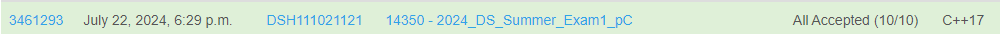
\includegraphics[width=\textwidth]{pC_AC}
\end{figure}




\end{document}



\section*{pD}
\subsection*{AC作法}
建立一個 vector , 其中 index 代表的是經過的站, value 表示需要的油量。一開始把 $V$ 設為 index = 0 的油量,之後每讀取一次,就把前一次的油量加上這次的油量存起來
\subsection*{Time Complexity}
\subsection*{考試時沒有AC的原因}
寫pA和pB花的時間太多,所以後面兩題來不及寫。
\subsection*{AC截圖}